%
% File naacl2019.tex
%
%% Based on the style files for ACL 2018 and NAACL 2018, which were
%% Based on the style files for ACL-2015, with some improvements
%%  taken from the NAACL-2016 style
%% Based on the style files for ACL-2014, which were, in turn,
%% based on ACL-2013, ACL-2012, ACL-2011, ACL-2010, ACL-IJCNLP-2009,
%% EACL-2009, IJCNLP-2008...
%% Based on the style files for EACL 2006 by 
%%e.agirre@ehu.es or Sergi.Balari@uab.es
%% and that of ACL 08 by Joakim Nivre and Noah Smith

\documentclass[11pt,a4paper]{article}
\usepackage[hyperref]{naaclhlt2019}
\usepackage{times}
\usepackage{latexsym}
% \usepackage[pagebackref,breaklinks,colorlinks]{hyperref}
\usepackage{url}
\usepackage{graphicx}
\usepackage{adjustbox}

\aclfinalcopy % Uncomment this line for the final submission
%\def\aclpaperid{***} %  Enter the acl Paper ID here

%\setlength\titlebox{5cm}
% You can expand the titlebox if you need extra space
% to show all the authors. Please do not make the titlebox
% smaller than 5cm (the original size); we will check this
% in the camera-ready version and ask you to change it back.

\newcommand\BibTeX{B{\sc ib}\TeX}

\title{Research Paper Summarizer}

\author{Afnan Mir \\
  amm23523 \\
  {\tt afnanmir@utexas.edu} \\\And
  Jaykumar Patel \\
  jnp2369 \\
  {\tt patel.jay4802@utexas.edu} \\}

\date{\today}

\begin{document}
\maketitle
\begin{abstract}
  In this report, we aim to improve accessibility of information presented in complex research papers by using Natural Language Processing (NLP) methods to automatically generate summaries of research papers that are easier to read than the average technical abstract. A dataset of research papers in the medical field which have a technical abstract as well as a plain language summary associated with each paper was used to finetune a pretrained T5 model. The research paper and the technical abstract were used as inputs to the model, and the plain language summary was used as the target output. The finetuned model was evaluated using the ROUGE metric for summarization as well as various readability metrics such as Flesch and Dale Chall. Human evaluation was also used. Our code can be found \href{https://github.com/afnanmmir/Research-Paper-Summarizer}{here}.
\end{abstract}

\section{Introduction}

\indent \indent Research papers are groundbreaking in terms of presenting new findings, theories, and perspectives, making them essential for scientific breakthroughs. However, the knowledge presented in research papers is often inaccessible to the general public for various reasons. Reasons include putting research papers behind paywalls, using dense technical language that the average person cannot understand, and sometimes simply being far too long. This discourages those in the general public who may be interested in the topic of the research paper or those who would like to enter the research area presented in the paper from reading the paper. Though the first issue is not one that can be solved without a change in the current publishing system, the latter two issues can be addressed by using Natural Language Processing (NLP) methods to automatically generate summaries of research papers that are easier to read than the average technical abstract. This would involve finetuning a pretrained model on a dataset to convert the paper and its technical abstract into a plain language summary, which, to some extent, would take down the barrier of technical language and length.
\section{Dataset and Resources}
\subsection{Dataset}
\indent \indent To train and evaluate the model, a dataset of research papers in the biomedical domain was used. This dataset contains 28,124 research papers, each with an associated technical abstract and a plain language summary. The technical abstract is the abstract that is typically found in research papers, but the plain language summary is a summary that is written by the author, where they are required to highlight how the work fits into a broader context in a simple manner without complex acronyms and terminology \cite{luo2022readability}. The dataset was split into the train set, the validation set, and the test set, with 26,124, 1,000, and 1,000 papers respectively. The dataset can be found \href{https://www.dropbox.
com/s/huwm01glsk9fou0/plos_readability_ctrl_sum_
corpus.rar?dl=0}{here}.

\subsection{Model Resources}

\indent \indent To obtain the resources to load our pretrained model and finetune it, \href{https://huggingface.co/}{HuggingFace} was used, which is an online hub where users and/or companies are able to publish their trained PyTorch or TensorFlow models for others to use. HuggingFace provides a high-level API that allows us to load the model, load the dataset in a proper format, and train the model without worrying about the inner workings of the model.

In order to train the model efficiently, training on a local machine would not suffice. For this purpose, \href{colab.research.google.com}{Google Colab} was used, where the access of a GPU is provided for free for some limited amount of time.

\section{Methodology}

\subsection{Model Selection}
\indent \indent For the summarization task, a couple of model architectures were researched and explored. The final architecture that was chosen was an encoder-decoder transformer model; namely the T5 (Text-to-Text Transfer Transformer) model \cite{raffel2020exploring}. This model was pretrained on a mixture of self-supervised and supervised tasks over a large text corpus, which made it a well-performing model for a variety of tasks out of the box. All that had to be done was the prepend the input with the given task (e.g., for summarization: "summarize: ", for translation: "translate English to German: "). The model was chosen because of its ease of use as well as its performance on the general summarization task.

\subsection{Model Finetuning/Training}
\indent \indent To finetune the model, first the data had to be prepared. The initial approach was to use the LongT5 model, which was specialized for tasks with long inputs, and provide as much of each research paper as possible as the input to the model \cite{guo2022longt5}. However, due to the limited resources provided by Google Colab, it became apparent that using whole research papers as the input to the model would not be possible without running out of GPU memory or truncating our inputs to the point that significant information was lost. Therefore, the approach was changed to use the base T5 model and provide the technical abstract as the input to hopefully create a readable summary.


The data was converted into input tokens that are digestable by the model using the HuggingFace Tokenizer API. The model was then trained using the HuggingFace Trainer API, which allows for easy training of a model on a dataset\footnote{Both of the API's can are found in the Transformers library: \url{https://github.com/huggingface/transformers}}. The model was trained for 3 epochs, with a learning rate of 2e-5, a maximum input length of 1024 tokens, and a maximum output length of 256 tokens. The training for this would take around 5 hours in the Google Colab environment.

\subsection{Summary Generation}
\indent \indent Once the model was finetuned, it was used to generate summaries for the test set. Initially, the default parameters were used for the generation of the summaries; however, using these parameters led to the generation of summaries that were not very readable for many reasons. One main reason was the constant generation of repeated tokens as seen in the following example: \\
\texttt{Schistosoma mansoni is one of the major tropical infectious diseases responsible for tropical infectious diseases caused by Schistosoma mansoni Schistosoma Mansoni Schistosoma Mansoni Schistosoma Mansoni Schistosoma Mansoni Schistosoma Mansoni Schistosoma Mansoni Schistosoma Mansoni Schistosoma Mansoni Schistosoma Mansoni}. \\
This case happened quite often in the test set. To mitigate these issues, the following parameters were used for the generation of the summaries: \\
\texttt{max\_length=256, min\_length=64, no\_repeat\_ngram\_size=2, num\_beams=4, early\_stopping=True, length\_penalty=2.0}. \\
Parameters like \texttt{length\_penalty} and \texttt{early\_stopping} prevented the model from generating summaries that were too long because the longer the summaries went, the more susceptible they were to becoming unreadable. The \texttt{no\_repeat\_ngrame\_size} parameter was implemented to make sure that the model did not generate the same token over and over again. With the implementation of these parameters, the summaries generated by the model were far more readable and coherent.


\section{Results and Evaluation}

% \indent \indent Describe as clearly as possible what it is your system can and cannot do. You can show examples of things your system is getting correct and of errors it is making. If applicable, measure performance by some performance metric.

\indent \indent The performance of the model was evaluated on two main factors: the readability and the quality of the summaries generated, and these evaluations were done using two primary methods. The first method was to utilize conventional numerical metrics to evaluate the model's performance. To evaluate readability, the Flesch and Dale Chall readability metrics were used \cite{Flesch1948}, \cite{chall1995readability}. To evaluate the quality of the summaries, the Rouge1, Rouge2, and RougeL metrics were used \cite{lin-2004-rouge}. Our second primary method was to use human evaluation to evaluate the readability and the quality of the generated summaries.

\subsection{Metrics}

\indent \indent After running the various metrics, here are the results of the predicted summaries compared to the original abstracts and original summaries. Although the original text performed better than the predicted text, the predicted text was fairly close in metrics such as Dale Chall, which measures the difficulty of the words in the text, as well as Rouge1 and Rouge2 which specifically looks at the overlap of unigrams and bigrams respectively. The Rouge metrics were compared to the original Rouge scores generated in the original paper this dataset was used in \cite{luo2022readability}. The results of the metrics are shown in the following table:

\begin{table}
  \begin{center}
    \begin{adjustbox}{width=0.49\textwidth}
      \begin{tabular}{|c | c | c | c|} 
      \hline
      Metrics Averaged & Predicted Summaries & Original Abstracts & Original Summaries \\ [1ex] 
      \hline\hline
      Flesch & 16.8523 & 27.4492 & 29.3275 \\ [1ex]
      \hline
      Dale Chall & 12.2706 & 11.0360 & 10.8992 \\ [1ex]
      \hline
      Dale Chall v2 & 10.8840 & 9.6439 & 9.7807 \\ [1ex]
      \hline
      Rouge1 & 0.4036 & 0.4987 & 0.4731 \\ [1ex]
      \hline
      Rouge2 & 0.1249 & 0.1785 & 0.1473 \\ [1ex] 
      \hline
      RougeL & 0.2140 & 0.4602 & 0.4308 \\ [1ex] 
      \hline
      \end{tabular}
  \end{adjustbox}
  \end{center}
\end{table}    


\subsection{Human Evaluation}

\indent \indent As aforementioned, the second method for evaluating results was using human evaluation. This involved showing an evaluator a predicted summary and the technical abstract side by side. The specific side that the text was shown on was randomized. Then the evaluator would select which side they thought was easier to read. Here are the results:

% \begin{figure}[!htbp]
  % \centering
  % 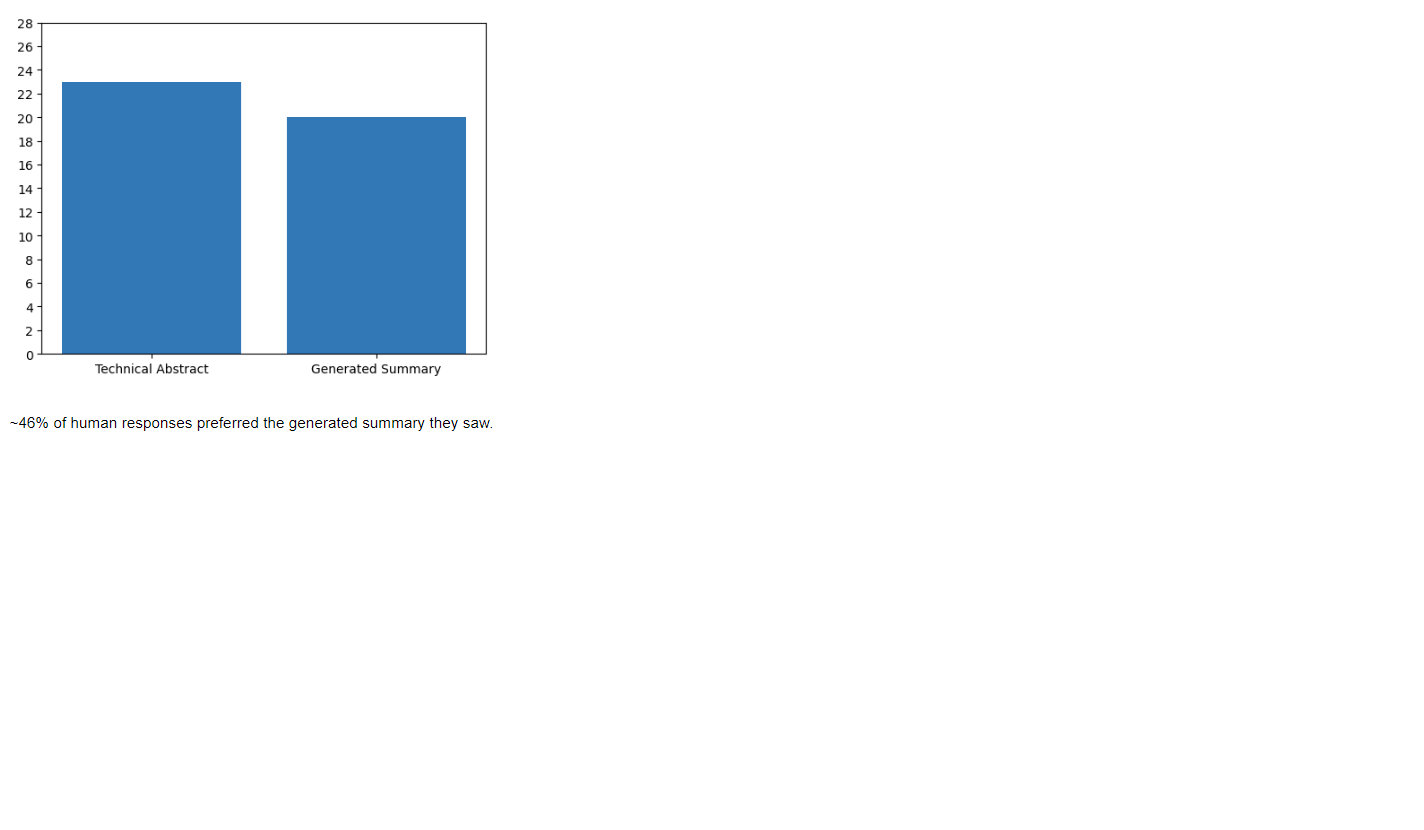
\includegraphics[width=500pt, height=300pt]{human_evaluation_results.png}
  % \caption{Human Evaluation Results}
% \end{figure}

\begin{table}[!htbp]
  \begin{tabular}{|c | c|} 
   \hline
   Text & Votes \\ [1ex] 
   \hline\hline
   Technical Abstract & 23 \\ [1ex]
   \hline
   Generated Summaries & 20 \\ [1ex]
   \hline
  \end{tabular}
\end{table}


\indent \indent As shown above, approximately 46\% humans preferred the generated summaries over the technical abstracts. This is a fairly good result, considering that the model was only trained for 3 epochs, and the model was only finetuned on a small subset of the data. With more training and more data, the model may be able to perform better.

\subsection{Model Shortcomings}
\indent \indent Though these evaluations are somewhat promising, digging deeper into the model showed some very obvious shortcomings. First, one thing that was very apparent was the fact that for some of the technical abstract, the model would end up generating the same exact abstract as the output minus a few sentences in between. Though removing some sentences may make an abstract more "readable", that is not the intent of the model. It is supposed to reword the abstract entirely to make it more readable. Additionally, there would be some cases of "hallucinations" from the model, where in the summary, the model would generate information that was either not in the technical abstract or was completely false. This is a very big issue, as even though readability may improve, this would not matter if the information in the summary is false.

A bottleneck that may have led to many of these issues was the lack of resources we had available. Only a limited amount of GPU memory and time was provided in the Google Colab environment, making it difficult to train a model effectively to perform this task.

\section{Future Work}

\indent \indent Upon reflection, there were a few evident reasons for the performance of the model. Firstly, the model was only trained on the technical abstracts, which limited the information the predicted summaries was able to capture. Thus, as next steps, the model would be trained on the techncal abstract as well as the introduction and the conclusion of the paper allowing the model to capture more information. Secondly, the model was only trained for 3 epochs, which is not enough to capture the nuances of the data. Thus, the model would be trained for more epochs. Lastly, other metrics would be used to evaluate the model, such as the RNPTC metric \cite{luo2022readability}.

\appendix

\section{Group Work Split}
For this project, Afnan took responsibility of formatting the data properly to be ingested by the model. He also took responsibility of training the model on Google Colab. Jaykumar took responsibility of generating the summaries for the test set, which also included tuning the parameters of the finetuned model to generate the most coherent model. He also worked on creating the demo for the class presentation. Both Afnan and Jaykumar worked on performing the evaluation of the summaries generated, and they both worked on the presentation and writing the

\bibliography{naaclhlt2019}
\bibliographystyle{acl_natbib}




\end{document}
